% THIS IS SIGPROC-SP.TEX - VERSION 3.1
% WORKS WITH V3.2SP OF ACM_PROC_ARTICLE-SP.CLS
% APRIL 2009
%
% It is an example file showing how to use the 'acm_proc_article-sp.cls' V3.2SP
% LaTeX2e document class file for Conference Proceedings submissions.
% ----------------------------------------------------------------------------------------------------------------
% This .tex file (and associated .cls V3.2SP) *DOES NOT* produce:
%       1) The Permission Statement
%       2) The Conference (location) Info information
%       3) The Copyright Line with ACM data
%       4) Page numbering
% ---------------------------------------------------------------------------------------------------------------
% It is an example which *does* use the .bib file (from which the .bbl file
% is produced).
% REMEMBER HOWEVER: After having produced the .bbl file,
% and prior to final submission,
% you need to 'insert'  your .bbl file into your source .tex file so as to provide
% ONE 'self-contained' source file.
%
% Questions regarding SIGS should be sent to
% Adrienne Griscti ---> griscti@acm.org
%
% Questions/suggestions regarding the guidelines, .tex and .cls files, etc. to
% Gerald Murray ---> murray@hq.acm.org
%
% For tracking purposes - this is V3.1SP - APRIL 2009

\documentclass{acm_proc_article-sp}

\usepackage[utf8]{inputenc}
\usepackage{graphicx}
\usepackage{caption}

\begin{document}

\title{Une étude des covert channels}

%\subtitle{[Extended Abstract]
%\titlenote{A full version of this paper is available as
%\textit{Author's Guide to Preparing ACM SIG Proceedings Using
%\LaTeX$2_\epsilon$\ and BibTeX} at
%\texttt{www.acm.org/eaddress.htm}}}

%
% You need the command \numberofauthors to handle the 'placement
% and alignment' of the authors beneath the title.
%
% For aesthetic reasons, we recommend 'three authors at a time'
% i.e. three 'name/affiliation blocks' be placed beneath the title.
%
% NOTE: You are NOT restricted in how many 'rows' of
% "name/affiliations" may appear. We just ask that you restrict
% the number of 'columns' to three.
%
% Because of the available 'opening page real-estate'
% we ask you to refrain from putting more than six authors
% (two rows with three columns) beneath the article title.
% More than six makes the first-page appear very cluttered indeed.
%
% Use the \alignauthor commands to handle the names
% and affiliations for an 'aesthetic maximum' of six authors.
% Add names, affiliations, addresses for
% the seventh etc. author(s) as the argument for the
% \additionalauthors command.
% These 'additional authors' will be output/set for you
% without further effort on your part as the last section in
% the body of your article BEFORE References or any Appendices.

\numberofauthors{2} %  in this sample file, there are a *total*
% of EIGHT authors. SIX appear on the 'first-page' (for formatting
% reasons) and the remaining two appear in the \additionalauthors section.
%
\author{
% You can go ahead and credit any number of authors here,
% e.g. one 'row of three' or two rows (consisting of one row of three
% and a second row of one, two or three).
%
% The command \alignauthor (no curly braces needed) should
% precede each author name, affiliation/snail-mail address and
% e-mail address. Additionally, tag each line of
% affiliation/address with \affaddr, and tag the
% e-mail address with \email.
%
% 1st. author
\alignauthor
Hoël Boëdec\\
       \affaddr{ENSIMAG - ISSC}\\
       \affaddr{3 rue Amiral Courbet}\\
       \affaddr{Grenoble, France}\\
       \email{hoel.boedec@phelma.grenoble-inp.fr}
% 2nd. author
\alignauthor
Fournier Mickaël\\
       \affaddr{ENSIMAG - ISSC}\\
       \affaddr{22 rue Francis Jaquard}\\
       \affaddr{Grenoble, France}\\
       \email{mickael.fournier@phelma.grenoble-inp.fr}
}
% There's nothing stopping you putting the seventh, eighth, etc.
% author on the opening page (as the 'third row') but we ask,
% for aesthetic reasons that you place these 'additional authors'
% in the \additional authors block, viz.
% \additionalauthors{Additional authors: John Smith (The Th{\o}rv{\"a}ld Group,
% email: {\texttt{jsmith@affiliation.org}}) and Julius P.~Kumquat
% (The Kumquat Consortium, email: {\texttt{jpkumquat@consortium.net}}).}
% \date{30 July 1999}
% Just remember to make sure that the TOTAL number of authors
% is the number that will appear on the first page PLUS the
% number that will appear in the \additionalauthors section.

\maketitle
\begin{abstract}
    Un canal caché, covert channel en anglais, est un medium de communication permettant à plusieurs systèmes de transmettre de l'information de manière cachée.
    En effet, à l'inverse d'une communication encryptée où le seul but est de rendre l'information illisible par un attaquant, l'utilisation d'un covert channel a pour but de cacher l'existence même de toute communication suspecte. On comprendra aisément l'intérêt de ce type de communication lorsqu'il s'agit de communiquer en temps de guerre, ou lorsque des hackers préparent une attaque DDoS synchronisée par exemple. Le simple fait de détecter le passage de messages encryptés peut réveler à l'ennemi l'imminence d'une attaque.\\
    Par ailleurs, le développement des réseaux à haute bande passante permet de créer des covert channels à débit de plus en plus important.
    Les types de covert channels pouvant être aussi variés que l'imagination de leurs utilisateurs, ceci peut les rendre extrêmement difficiles à détecter.\\
    Le Département de la Défense des États-Unis énonce une liste de critères dans le Trusted Computer System Evaluation Criteria (TCSEC) afin d'évaluer la sécurité d'un système informatique : l'analyse des covert channels intervient dans un système de niveau B2/B3.
\end{abstract}

% \terms{Theory}

\keywords{covert channel, steganography, data hidding} % NOT required for Proceedings

\section{Introduction}
Un exemple classique d'utilisation de covert channel est l'histoire de deux prisonniers : Alice et Bob.\\
Alice et Bob souhaitent se mettre d'accord sur l'heure de leur évasion, mais leur seul moyen de communication est Wendy, la gardienne, qui accepte de faire passer tout message non malicieux. Evidemment si Alice donne le message `15h30` à Wendy, cette dernière va surveiller Alice et Bob de très près à 15h30.`En revanche si Alice et Bob se sont mis d'accord sur un code au préalable, où tout mot ayant un nombre impair de lettre vaut 0, et les autres valent 1, Alice peut faire passer un message ayant l'air non-malicieux, mais transportant une information malicieuse.\\
Dans cet article nous rappellerons le principe de la stéganographie, puis les types de covert channels qui existent. Ensuite, nous explorerons l'exemple de rcovert pour, ensuite, s'intéresser aux méthodes de détection et à quelques exemples historiques.

\begin{figure}
\centering
\epsfig{file=Alice&Bob.eps, height=2in, width=4in}
\end{figure}

\section{Steganographie}
\subsection{Principe}
La steganographie est l'art de la dissimulation. Elle est comparée à la cryptographie qui est l'art du secret. Elle consiste à faire passer un message dans un autre message sans qu'une personne extérieure puisse le détecter. L'existence de l'échange de message doit rester secret.\\
L'efficacité de ce camouflage est intrinséquement limitée car il suffit de supprimer entièrement l'information et le message caché disparaitra avec le reste du message. Cependant, dans la société actuelle, l'échange d'information est indispensable. C'est pourquoi la steganographie restera toujours un moyen de dissimulation.\\
Ce message secret peut être par exemple caché dans une image, un texte ou encore un son.

\subsection{Exemples}
\subsubsection{Message transporté dans une image}
Le codage de la couleur d'une image se fait en triplé d'octets. Chaque octet de ce triplé regroupe des informations sur les niveaux de rouge, vert et bleu d'un pixel. Pour utiliser la steganographie dans une image il est d'usage de modifier le bit de poids faible de chaque couleur d'un pixel. Ainsi, le niveau de la couleur ne changera que d'un pas de 1 ce qui à l'oeil nu ne sera pas perceptible, alors que chaque bit de poids faibles contiendra de l'information utile à celui qui en connait l'existence.

\begin{figure}
\centering
\epsfig{file=Steganography_original.eps, height=1in, width=1in}
\caption{[Wikipedia] Image d'un arbre avec une image steganographiquement cachée. La photo cachée est révélée en ne gardant que les deux bits de poids faible de chaque couleur qui la compose. L'image cachée est visible ci-dessous.}
\end{figure}

\begin{figure}
\centering
\epsfig{file=Steganography_recovered.eps, height=1in, width=1in}
\caption{[Wikipedia] Image d'un chat extraite de l'image d'arbre ci-dessus.}
\end{figure}

\subsubsection{Message transporté dans un texte}
La stegnographie dans un texte peut être employée à travers deux procédés. Le premier consiste à modifier l'interlettrage. Aujourd'hui, grâce à nos imprimantes laser on peut modifier cet espace entre les lettres d'une façon si infime que l'oeil nu ne peut pas le détecter. Le décodage d'un message caché par ce procédé ne peut se faire que grâce à un ordinateur.\\
Le deuxième est plus simple à détecter pour un oeil avisé. Il s'agit de mettre un point en-dessous de lettres choisies dans un texte. Cependant ce procédé ne peut être efficace que pour des textes conséquents car sinon les points deviendraient trop visible et il y aurait plus de chance qu'une personne remarque cette anomalie.

\begin{center}
\includegraphics[height=7cm]{texte.png}
\captionof{figure}{Un texte tout à fait anodin}
\end{center}


\begin{center}
\includegraphics[height=7cm]{textcolor.jpg}
\captionof{figure}{Les informations cachées soient par différence de grosseur de lettre (bleu), soient par taille d'espaces différente (vert) soient par police différente (rouge)}
\end{center}

\subsection{Vers les covert channels}
La stéganographie permet de faire passer de l'information sans en révéler l'existence. C'est ce qui est la base des covert channels (canal caché).


\section{Types de Covert channel}
On distingue classiquement deux types de covert channels : les storage channels et les timing channels.

\subsection{Storage channels}
Un storage channel consiste à écrire l'information sensible à transmettre dans un endroit où le récepteur sera en mesure de récupérer l'information. L'exemple le plus classique de covert channel consiste à écrire l'information dans certains champs du protocole TCP (par exemple).\\
Une approche moins classique consiste à utiliser l'imperfection des canaux de transmission afin de créer un covert channel dans la couche physique des protocoles de communication sans fil. En effet, les canaux imparfaits introduisent du bruit dans les transmissions. Il est alors possible d'émettre un signal qui semble bruité, mais qui est en fait un signal volontairement distordu et qui transporte de l'information cachée.

\begin{center}
\includegraphics[height=3cm]{DirtyConstellation.eps}
\end{center}

Les exemples suivants sont issus de [citer Survey...]

\subsubsection{Utilisation des bits d'entête non-utilisés}
De nombreux covert channels utilisent des bits inutilisés ou réservés présents dans les entêtes des différents protocoles. En effet, si les valeurs standards ne sont pas précisées dans le protocole, il est possible de stocker l'information voulue dans ces champs. Les possibilités sont multiples, mais on peut citer l'exemple de l'utilisation du TCP Urgent Pointer comme covert channel. Celui-ci est en effet inutilisé si le bit URG n'est pas mis à 1.

\subsubsection{Utilisation d'extension d'entête ou de padding}
Certains protocoles permettent d'étendre les entêtes standards, parfois en autorisant la transmission de données arbitraires. Il est alors facile de transmettre de l'information sensible.
Si un protocole ne force pas le format des bits de padding, il est également possible de stocker le message directement dans le padding du paquet.

\subsubsection{Quelques autres méthodes}
    Pour une question de longueur nous ne développons pas le principe de toutes les méthodes existantes, mais voici une liste non-exhaustive issue de [Survey] énoncant les cibles potentielles d'un covert channel :
    \begin{itemize}
    \item IP Identification header field \& Fragment Offset
    \item TCP initial sequence number field
    \item Checksum field
    \item IP time to live field
    \item Address fields \& Packet lengths
    \end{itemize}

\subsection{Timing channels}
Un timing channel consiste à utiliser le temps comme système de modulation de l'information. L'émetteur module l'utilisation d'une ressource (utilisation CPU, simulation de bruit dans le canal, etc) en fonction du temps, alors que le récepteur observe l'intervalle entre chaque modification et en déduit l'information.
L'accès à un disque dur peut être un exemple de covert timing channel. Le receveur, ayant des droits d'accès au périphérique assez élevé pour voir les tentatives de lecture et, l'envoyeur, pouvant faire des demandes de lecture, peuvent communiquer à l'aide des intervalles de temps entre chaque tentative de lecture.\\
Pour reprendre l'exemple des prisonniers Alice et Bob, il leur est tout à fait possible d'utiliser Wendy comme un timing channel. Admettons qu'ils se soient, au préalable, mis d'accord sur le code suivant : tous les jours il y a deux possibilités, soit un message (ayant l'air innocent, comme "Bonjour") est transmis par Wendy entre les deux prisonniers, soit pas. Si un message est transmis, alors ce 'jour' vaut 1, sinon le 'jour' vaut 0. En découpant les jours par paquets de 8 il est alors possible de transmettre des caractères d'un prisonnier à l'autre, et il est donc possible pour eux de planifier leur évasion.
Cette méthode n'est qu'un exemple, mais montre la discrétion du procédé pour un oeil extérieur, et donc sa puissance.

\begin{figure}
\centering
\epsfig{file=Alice&Bob2.eps, height=2in, width=3in}
\end{figure}


\section{Exemple : rcovert}
\subsection{Principe}
Rcovert, Raw Covert, est un petit logiciel développé par deux ingénieurs d'Orange comme preuve d'utilisation d'un nouveau type de covert channel : la communication dissimulée d'informations dans des paquets ACK. Le principe est le suivant : les paquets ACK sont considérés par les réseaux comme des données sans risques et ne sont globalement pas surveillés. Ainsi, si il est possible de transmettre nos données dans un tel paquet alors il est possible de l'utiliser comme covert channel. Ce dernier est utilisé sur le protocole 802.11 est l'information utile est stockée dans le champ d'adresse RA (Receiver Adress).\\
Ce logiciel nécessite certaines configurations. Tout d'abord, il faut avoir un injection driver disponible qui permet d'injecter des paquets sur le réseau. Ensuite, l'interface wifi de l'ordinateur doit pouvoir être passé en mode monitor, qui est un mode permettant à l'ordinateur de pouvoir écouter tout le trafic du réseau wifi.

\subsection{Mesures}
D'après l'implémentation, la charge utile par paquet ACK s'élève à 1 octet. Sachant qu'on envoie un paquet toutes les 100ms, le débit de données utiles s'éléve à 10 octets par seconde, soit 10 caractères par seconde.

\subsection{Impact en pratique}
\subsubsection{Ping}
Au lieu d'utiliser par défaut le protocole ICMP avec les paquets echo/request afin de savoir si une machine est atteignable ou non, on peut utiliser les paquets ACK. Si une cible est atteinte par ce type de paquet cette dernière renverra un paquet RST, qui correspond en théorie à une rupture anormale de la connexion (reset).\\
En plus d'utiliser peu de traffic sur le réseau, les requêtes ACK peuvent être une bonne alternative quand l'utilisation du protocole ICMP n'est pas applicable à cause de filtrage de paquets ou de firewalls. En effet, comme on l'a dit précédemment les requêtes ACK à une machine sont relativement indétectables. 
\subsubsection{Nmap}
De même, dans la perspective de recherche de failles sur une machine, ce type de covert channel permet d'en scanner les ports et de savoir donc lesquels sont ouverts même en cas de présence d'un firewall par exemple.


\section{Au-delà de rcovert}

\subsection{Principal problème : le bruit}
Comme nous l'avons vu précedemment, le bruit peut être utilisé pour mettre en place un canal caché au niveau de la couche physique.\\
Néanmoins le bruit peut également devenir un véritable ennemi pour les covert channels.
[citer "an overview of covert channels]
En effet, un bruit suffisant peut provoquer des erreurs dans le signal reçu, obligeant donc le récepteur à demander le renvoi des informations plusieurs fois, jusqu'à ce qu'il soit sûr que l'information reçue est fiable. Ceci ralentit alors drastiquement la vitesse de communication et rend donc le covert channel bien moins efficace.

\subsection{Une méthode de détection}
Notre étude précédente des storage channels nous a montré que plus l'espace disponible dans les champs des protocoles utilisés est grand, plus le covert channel peut envoyer d'information par paquet émis. Notons d'ailleurs qu'un covert channel qui ne ferait passer qu'un seul bit malicieux par paquet serait en mesure d'extraire 26GB de données en une année. [citation Survey of covert...]\\
Afin de détecter ce traffic, il convient de limiter les champs non-surveillés dans les protocoles utilisés. Une politique de détection de covert channel correcte permet de limiter la quantité d'information transmise par paquet, et donc de forcer les attaquants à augmenter le nombre de messages envoyés. Il est alors bien plus facile pour les administrateurs réseaux de détecter les activités suspectes.


%\subsection{Comparaison entre différents médiums de transmission (avantages, désavantages)}
%\subsubsection{Champ d'identification des paquets IP}
%\subsubsection{Champ du nombre de séquence initial des paquets TCP}
%\subsubsection{Champ du nombre de séquence de ACK des paquets TCP}

\subsection{Débit des covert channels}
Un covert channel est usuellement considéré à 'grande' bande passante si son débit excède 100 bits par seconde. A l'inverse et d'après le Orange Book, les covert channels dont le débit est inférieur à 1 bit par seconde sont considérés comme acceptables dans la plupart des environnements de travail.\\
D'après [Attacks with Stegano] il est possible de cacher jusqu'à 77 bits par MAC data frame, permettant ainsi la création d'un covert channel à grande bande passante.

\subsection{Contre-mesure}
La contre mesure la plus naturelle serait de surveiller toute la data qui circule sur le réseau. Une entreprise américaine WebStone Tehnologies avaient d'ailleurs lancé leur propre service de surveillance basé sur la steganographie. Ce dernier s'appuyait sur un modèle mathématique qui essayait de déterminer si une information était dissimulée ou non.\\
Le problème de cette méthode est qu'elle ralentit considérablement les systèmes surveillés. En effet, comme le rappelle [Survey] la plupart du temps un covert channel ne peut être completement effacé que si l'on remplace les procédures automatiques par des procédures manuelles. Ceci n'étant pas envisagable il ne faut pas espèrer avoir un système exempt de covert channel, mais un système qui limite au maximum l'exploitation des covert channels.\\
Voici quelques mesures proposées par [Survey] afin d'éliminer ou de limiter les covert channels.

\subsubsection{Sécuriser les hôtes}
Pour qu'un covert channel d'exfiltration de données puisse être établi il faut nécessairement compromettre une machine (Trojan, etc). Si l'hôte est correctement sécurisé la mise en place d'un covert channel est alors fortement compromise.

\subsubsection{Normaliser le traffic qui passe sur le réseau}
On a vu précédemment qu'il était possible d'utiliser des bits réservés ou non-utilisés pour créer un covert channel. Si ces champs sont normalisés à un endroit quelconque du réseau ces coverts channels seront éliminés.

\subsubsection{Limiter la capacité du covert channel}
Il est possible de limiter la capacité du covert channel en introduisant du bruit dans le canal. En connaissant le débit maximum du covert channel et le débit de fuite d'informations que l'on peut tolèrer pour un système, il est possible d'ajuster l'introduction de bruit pour conserver un système le plus performant possible.

\subsection{Faits historiques et illustration pratique}
\subsubsection{Al-Quaeda}
Après les attentats du 11 Septembre 2001, les autorités américaines ont affirmé que des membres du groupe Al-Qaeda, ainsi que d'autres groupes terroristes ont eu recours à la steganographie. Les covert channels utilisés étaient des images (sites pornographiques) et du texte (chat de sport).

\subsubsection{Les services secrets Russes}
D'après le FBI, les services secrets Russes utilisent les images afin de pouvoir communiquer avec des agents secrets implantés à l'étranger.

\subsubsection{Imprimantes lasers}
De nombreuses imprimantes lasers utilisent la steganographie afin de cacher des informations telles que le numéro de série de l'utilisateur ou encore la date et l'heure de l'impression. 


\section{Conclusion}
Dans cet article nous avons tout d'abord présenté le principe de la stéganographie, art de la dissimulation, et son lien direct avec les covert channels. Nous avons ensuite décrit les deux grands types de covert channel : les storage channels et les timing channels. Nous avons ensuite brievement abordé l'exemple de rcovert, une implémentation de covert channel réalisée par deux ingénieurs d'Orange labs. Enfin, nous avons exploré les limites des covert channels (comme le bruit), ainsi que des méthodes afin de les détecter, puis nous avons donné quelques exemples de l'utilisation de covert channel et quelques faits historiques.




%
% The following two commands are all you need in the
% initial runs of your .tex file to
% produce the bibliography for the citations in your paper.
% \bibliographystyle{abbrv}
% \bibliography{sigproc}  % sigproc.bib is the name of the Bibliography in this case
% \nocite{*}
% You must have a proper ".bib" file
%  and remember to run:
% latex bibtex latex latex
% to resolve all references
%
% ACM needs 'a single self-contained file'!
%

\bibliographystyle{abbrv}
\bibliography{sigproc}  % sigproc.bib is the name of the Bibliography in this case
\nocite{*}

\balancecolumns
% That's all folks!
\end{document}
